\documentclass{article}
\usepackage[T1]{fontenc} %%%key to get copy and paste for the code!
\usepackage[utf8]{inputenc} %%% to support copy and paste with accents for frnehc stuff
\usepackage{times}
\usepackage[scaled=0.85]{helvet}
\usepackage{graphicx}
\usepackage{ifthen}
\usepackage{xspace}
\usepackage{alltt}
\usepackage{latexsym}
\usepackage{url}            
\usepackage{amssymb}
\usepackage{amsfonts}
\usepackage{amsmath}
\usepackage{stmaryrd}
\usepackage{enumerate}
\usepackage{cite}
\usepackage[pdftex,colorlinks=true,pdfstartview=FitV,linkcolor=blue,citecolor=blue,urlcolor=blue]{hyperref}
\usepackage{xspace}

\usepackage{float}
% \usepackage{xcolor}
% \usepackage{listings}
% \usepackage{highlight}

\newboolean{showcomments}
\setboolean{showcomments}{true}
\ifthenelse{\boolean{showcomments}}
  {\newcommand{\bnote}[2]{
	\fbox{\bfseries\sffamily\scriptsize#1}
    {\sf\small$\blacktriangleright$\textit{#2}$\blacktriangleleft$}
    % \marginpar{\fbox{\bfseries\sffamily#1}}
   }
   \newcommand{\cvsversion}{\emph{\scriptsize$-$Id: macros.tex,v 1.1.1.1 2007/02/28 13:43:36 bergel Exp $-$}}
  }
  {\newcommand{\bnote}[2]{}
   \newcommand{\cvsversion}{}
  } 


\newcommand{\here}{\bnote{***}{CONTINUE HERE}}
\newcommand{\nb}[1]{\bnote{NB}{#1}}

\newcommand{\fix}[1]{\bnote{FIX}{#1}}
%%%% add your own macros 

\newcommand{\ab}[1]{\bnote{Alex}{#1}}
\newcommand{\sd}[1]{\bnote{Stef}{#1}}
\newcommand{\ja}[1]{\bnote{Jannik}{#1}}
\newcommand{\md}[1]{\bnote{MD}{#1}}
\newcommand{\jr}[1]{\bnote{JRe}{#1}}
\newcommand{\lf}[1]{\bnote{Luc}{#1}}

\graphicspath{{figures/}}
%%% 


\newcommand{\figref}[1]{Figure~\ref{fig:#1}}
\newcommand{\figlabel}[1]{\label{fig:#1}}
\newcommand{\tabref}[1]{Table~\ref{tab:#1}}
\newcommand{\layout}[1]{#1}
\newcommand{\commented}[1]{}
\newcommand{\secref}[1]{Section \ref{sec:#1}}
\newcommand{\seclabel}[1]{\label{sec:#1}}

%\newcommand{\ct}[1]{\textsf{#1}}
\newcommand{\stCode}[1]{\textsf{#1}}
\newcommand{\stMethod}[1]{\textsf{#1}}
\newcommand{\sep}{\texttt{>>}\xspace}
\newcommand{\stAssoc}{\texttt{->}\xspace}

\newcommand{\stBar}{$\mid$}
\newcommand{\stSelector}{$\gg$}
\newcommand{\ret}{\^{}}
\newcommand{\msup}{$>$}
%\newcommand{\ret}{$\uparrow$\xspace}

\newcommand{\myparagraph}[1]{\noindent\textbf{#1.}}
\newcommand{\eg}{\emph{e.g.,}\xspace}
\newcommand{\ie}{\emph{i.e.,}\xspace}
\newcommand{\etal}{\emph{et al.,}\xspace}
\newcommand{\ct}[1]{{\textsf{#1}}\xspace}


\newenvironment{code}
    {\begin{alltt}\sffamily}
    {\end{alltt}\normalsize}

\newcommand{\defaultScale}{0.55}
\newcommand{\pic}[3]{
   \begin{figure}[h]
   \begin{center}
   \includegraphics[scale=\defaultScale]{#1}
   \caption{#2}
   \label{#3}
   \end{center}
   \end{figure}
}

\newcommand{\twocolumnpic}[3]{
   \begin{figure*}[!ht]
   \begin{center}
   \includegraphics[scale=\defaultScale]{#1}
   \caption{#2}
   \label{#3}
   \end{center}
   \end{figure*}}

\newcommand{\infe}{$<$}
\newcommand{\supe}{$\rightarrow$\xspace}
\newcommand{\di}{$\gg$\xspace}
\newcommand{\adhoc}{\textit{ad-hoc}\xspace}

\usepackage{url}            
\makeatletter
\def\url@leostyle{%
  \@ifundefined{selectfont}{\def\UrlFont{\sf}}{\def\UrlFont{\small\sffamily}}}
\makeatother
% Now actually use the newly defined style.
\urlstyle{leo}



\title{Exploratory Data Analysis in Pharo}
\author{
  Oleksandr Zaytsev\\
  \texttt{olk.zaytsev@gmail.com}
}
\date{}

\begin{document}
\maketitle

%\title{Title that Describes the Contribution that Solves a Problem}
%\author{Oleksandr Zaytsev}
%\date{\today}
%\maketitle

\begin{abstract}
In this context...
We consider this problem P...
P is a problem because...
We propose this solution...
Our solution solves P in such and such way.

Pharo does not have the proper tools for data analysis. One of the most important tools is data frames - tabular data structures for data analysis. In this paper I demonstrate how the existing DataFrame can already be used for exploratory data analysis.
\end{abstract}


\section{Introduction}
\label{sec:intro}

Context

Problem

Explanatory data analysis is the ...

Known tracks for \sd{solutions}
	here you want to show that you are not an idiot not knowing what have been around

What our solution is \ct{Set} and \ct{OrderedCollection} (so that the reader knows where the paper is going)

Contribution of the paper

\paragraph{Paper structure} In the first section I provide a brief introduction into the explanatory data analysis. What is it good for? How to do it right? I will also provide you with all the basic knowledge about statistics and data analysis, such as statistical variable, types of variables etc. In the second section I briefly describe the DataFrame - new data structure for data analysis. In the following section I will give a step-by-step example of how to perform EDA on the well-known Iris data set.




\section{Problem Description}
\label{sec:problem}

Context, exposed with the \textbf{most precise terms possible} (don't open
unwanted doors for the reader)

Probably set the vocabulary before to cut any misinterpretation

Constraints that influenced the solution (because the solution is not
universal) \emph{e.g.} our requirements for a solution, possibly not all
satisfied. They should be sound and believable. Analysis of the criteria.
Imagine that you are another guy having this problem do the constraint
matches yours so that you could apply the solution

Problem

Factual solution tracks, to position...
Our solution in a nutshell.

\section{Exploratory Data Analysis (EDA)}
\label{sec:eda}

Here are the main reasons we use EDA:
\begin{itemize}
  \item detection of mistakes
  \item checking of assumptions
  \item preliminary selection of appropriate models
  \item determining relationships among the explanatory variables
  \item assessing the direction and rough size of relationships between explanatory and outcome variables
\end{itemize}


\section{DataFrame class}
\label{sec:dataframe}
...

%\section{Proposed Solution}%
\section{Exploring Iris Data Set}
\label{sec:contribution}

Free form, variable number of sections, technical details.

But in general do not mix solution and discussions/possible variation
let that for discussion

We can start by loading iris data set from a CSV file.
\begin{code}{}
data := DataFrame fromCsv: '/path/to/iris.csv'.
\end{code}

Now let's take a look at the first and the last 5 entries in our table. These slices are called \textit{head} and \textit{tail} of a data frame.

\begin{code}{}
data head.
data tail.
\end{code}

\subsection{Univariate non-graphical EDA}
To access a single variable we ask a data frame for a specific column, using its name or integer index

\begin{code}{}
var := data column: #sepal_width. "Accessing column by its name"
var := data columnAt: 1. "Getting column by index"
\end{code}

What we can do with a column depends on a type of statistical variable it represents. If the variable is categorical, we can ..., if its quantitative, we can look at the ... statistics.

\begin{code}{}
var min.
var max.
var range.
var average. "a.k.a. mean"
var median.
var mode.
var stdev.
\end{code}

\subsection{Univariate graphical EDA}
\subsubsection{Categorical}

Histogram is the only graphical technique that can be used for a categorical variable.

\begin{code}{}
var := data column: #species.
var barplot.
\end{code}

\begin{figure}[H]
  \begin{center}
  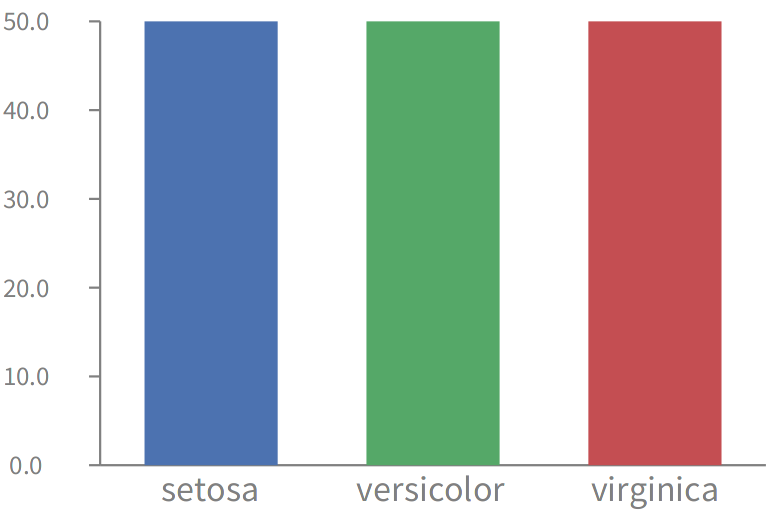
\includegraphics[width=0.75\linewidth]{species_bar}
  \end{center}
\end{figure}

\subsection{Multivariate non-graphical EDA}
...

\subsection{Multivariate graphical EDA}
\begin{figure}[H]
  \begin{center}
  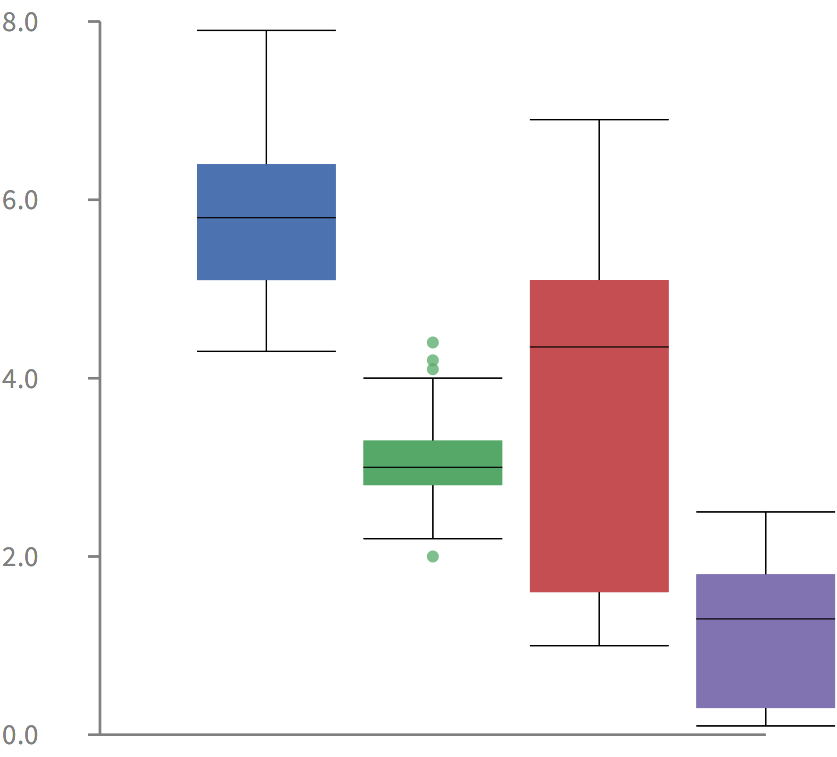
\includegraphics[width=0.75\linewidth]{boxplot}
  \caption{no need to put the file extension!}
  \end{center}
\end{figure}

\begin{figure}[!htp]
  \begin{center}
  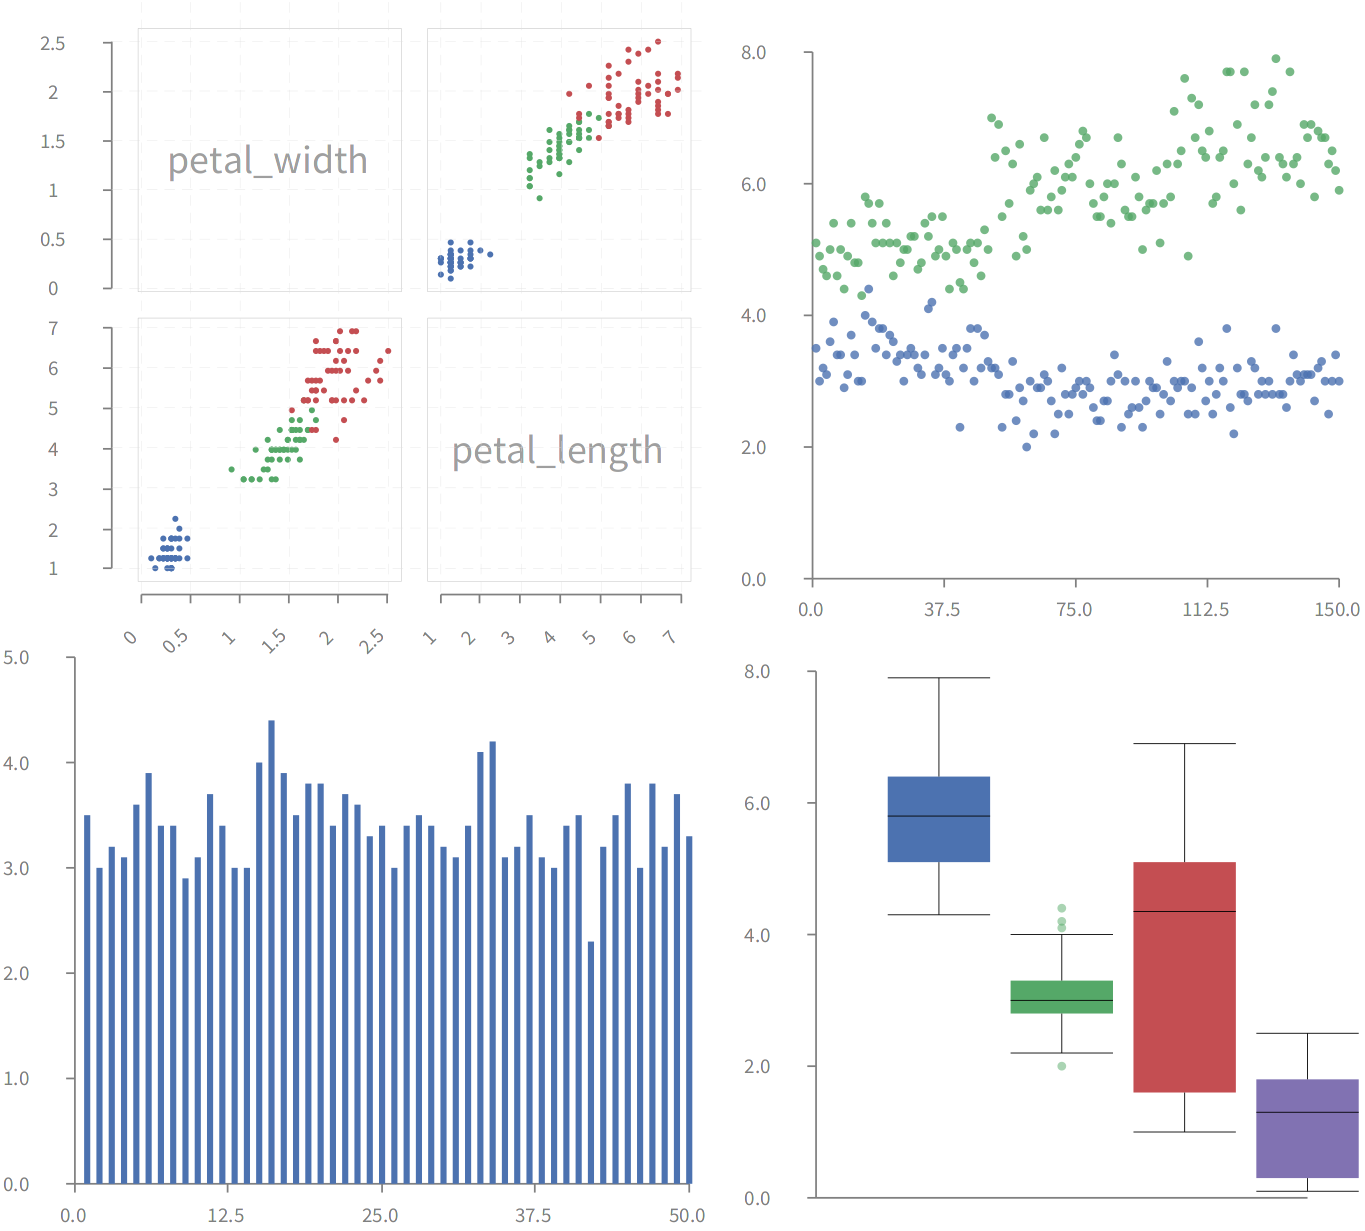
\includegraphics[width=\linewidth]{all_plots}
  \caption{no need to put the file extension!}
  \end{center}
\end{figure}


\section{Discussion}
\label{sec:discussion}

Discussion of actual solution \emph{vs.} initial constraints from
\ref{sec:problem}. Explain the space of the solution, why we made it this way.

Evaluation of the solution. How does the solution meet the criteria? Where
does it succeed or fails...


\section{Related Works}
\label{sec:related}

Other solutions in the domain, and a real comparison of our contribution with
solutions from other people.


\section{Conclusion}
\label{sec:conclusion}

In this paper, we \textsf{looked}\xspace at problem P with this context and these
constraints. We proposed solution S. It has such good points and such not so
good ones. Now we could do this or that.


% \section*{macro example}
%
% \ct{look at it this is code }
% \begin{code}{}
% Class>>nknkjbkjbkjb
%     \{| grgr | 
%     grgrgrgg 
%     a := 
% \end{code}

\subsection*{Acknowledgements} This work was supported by Ministry of Higher Education and Research, Nord-Pas de Calais Regional Council, FEDER through the 'Contrat de
Projets Etat Region (CPER) 2007-2013',  the Cutter ANR project, ANR-10-BLAN-0219 and the MEALS Marie Curie Actions program FP7-PEOPLE-2011-
IRSES MEALS (no. 295261). 

% \bibliographystyle{plain}
% \bibliography{foo.bib}

% \appendix
% 
% \section{Lots of Furry Technical Details}

\bibliographystyle{abbrv}
\bibliography{rmod,others}
\end{document}

%%% Local Variables: 
%%% coding: utf-8
%%% mode: latex
%%% TeX-master: "main"
%%% TeX-PDF-mode: t
%%% End:
